
% ----------------------------------------------------------------------
%                   LATEX TEMPLATE FOR PhD THESIS
% ----------------------------------------------------------------------

% based on Harish Bhanderi's PhD/MPhil template, then Uni Cambridge
% http://www-h.eng.cam.ac.uk/help/tpl/textprocessing/ThesisStyle/
% corrected and extended in 2007 by Jakob Suckale, then MPI-CBG PhD programme
% and made available through OpenWetWare.org - the free biology wiki


%: Style file for Latex
% Most style definitions are in the external file PhDthesisPSnPDF.
% In this template package, it can be found in ./Latex/Classes/
\documentclass[twoside,11pt]{Latex/Classes/PhDthesisPSnPDF}


%: Macro file for Latex
% Macros help you summarise frequently repeated Latex commands.
% Here, they are placed in an external file /Latex/Macros/MacroFile1.tex
% An macro that you may use frequently is the figuremacro (see introduction.tex)
% This file contains macros that can be called up from connected TeX files
% It helps to summarise repeated code, e.g. figure insertion (see below).

% insert a centered figure with caption and description
% parameters 1:filename, 2:title, 3:description and label
\newcommand{\figuremacro}[3]{
	\begin{figure}[htbp]
		\centering
		\includegraphics[width=1\textwidth]{#1}
		\caption[#2]{\textbf{#2} - #3}
		\label{#1}
	\end{figure}
}

% insert a centered figure with caption and description AND WIDTH
% parameters 1:filename, 2:title, 3:description and label, 4: textwidth
% textwidth 1 means as text, 0.5 means half the width of the text
\newcommand{\figuremacroW}[4]{
	\begin{figure}[htbp]
		\centering
		\includegraphics[width=#4\textwidth]{#1}
		\caption[#2]{\textbf{#2} - #3}
		\label{#1}
	\end{figure}
}

% inserts a figure with wrapped around text; only suitable for NARROW figs
% o is for outside on a double paged document; others: l, r, i(inside)
% text and figure will each be half of the document width
% note: long captions often crash with adjacent content; take care
% in general: above 2 macro produce more reliable layout
\newcommand{\figuremacroN}[3]{
	\begin{wrapfigure}{o}{0.5\textwidth}
		\centering
		\includegraphics[width=0.48\textwidth]{#1}
		\caption[#2]{{\small\textbf{#2} - #3}}
		\label{#1}
	\end{wrapfigure}
}

% predefined commands by Harish
\newcommand{\PdfPsText}[2]{
  \ifpdf
     #1
  \else
     #2
  \fi
}

\newcommand{\IncludeGraphicsH}[3]{
  \PdfPsText{\includegraphics[height=#2]{#1}}{\includegraphics[bb = #3, height=#2]{#1}}
}

\newcommand{\IncludeGraphicsW}[3]{
  \PdfPsText{\includegraphics[width=#2]{#1}}{\includegraphics[bb = #3, width=#2]{#1}}
}

\newcommand{\InsertFig}[3]{
  \begin{figure}[!htbp]
    \begin{center}
      \leavevmode
      #1
      \caption{#2}
      \label{#3}
    \end{center}
  \end{figure}
}


%%% Local Variables: 
%%% mode: latex
%%% TeX-master: "~/Documents/LaTeX/CUEDThesisPSnPDF/thesis"
%%% End: 

\usepackage[T1]{fontenc}
\usepackage{array}
\usepackage{pdfpages}
\usepackage{subfigure}
%\usepackage{graphics}
% or use the graphicx package for more complicated commands
%\usepackage{graphicx}

%: ----------------------------------------------------------------------
%:                  TITLE PAGE: name, degree,..
% ----------------------------------------------------------------------
\usepackage{graphicx}
\usepackage{booktabs}
%\usepackage{l3kernel}

      \textwidth 15cm
      \textheight 22cm
      \parindent 10pt
      \oddsidemargin 0.85cm
      \evensidemargin 0.37cm

\begin{document}

\thispagestyle{empty}

\begin{center}

Vrije Universiteit Amsterdam

\vspace{1mm}


\includegraphics[height=25mm]{0_frontmatter/figures/vu-griffioen}

\vspace{2cm}

{\Large Bachelor Thesis}

\vspace*{1.5cm}

\rule{.9\linewidth}{.6pt}\\[0.4cm]
{\huge \bfseries RDMA Key Value store:\\Scalability of RDMA transportation types \par}\vspace{0.4cm}
\rule{.9\linewidth}{.6pt}\\[1.5cm]

\vspace*{2mm}

{\Large
\begin{tabular}{l}
{\bf Author:} ~~Jan Erik (Jens) Troost ~~~~ (2656054)
\end{tabular}
}

\vspace*{2cm}

\begin{tabular}{ll}
{\it 1st supervisor:}   & ~~Dr. Animesh Trivedi \\
{\it daily supervisor:} & ~~supervisor name \\
{\it 2nd reader:}       & ~~supervisor name
\end{tabular}

\vspace*{2.5cm}

\textit{A thesis submitted in fulfillment of the requirements for\\the VU Bachelor of Science degree in Computer Science}

\vspace*{1.8cm}

\today\\[4cm] % Date

\end{center}

\newpage


% ----------------------------------------------------------------------
       
% turn of those nasty overfull and underfull hboxes
\hbadness=10000
\hfuzz=50pt


%: --------------------------------------------------------------
%:                  FRONT MATTER: dedications, abstract,..
% --------------------------------------------------------------


%\language{english}


% sets line spacing
\renewcommand\baselinestretch{1.2}
\baselineskip=18pt plus1pt


%: ----------------------- generate cover page ------------------------

%\begin{center}
%\textit{``I am the master of my fate, I am the captain of my soul'' \\ from {\em Invictus}, by William Ernest Henley}
%\end{center}

%: ----------------------- cover page back side ------------------------
% Your research institution may require reviewer names, etc.
% This cover back side is required by Dresden Med Fac; uncomment if needed.

%\newpage
%\vspace{10mm}
%1. First Reader: Name Surname
%
%\vspace{10mm}
%2. Daily Supervisor: Name Surname
%
%\vspace{10mm}
%3. Second Reader: Name Surname
%
%\vspace{10mm}
%4. Industrial Supervisor: Name Surname
%
%\vspace{20mm}
%Day of the defense:

%\vspace{20mm}
%\hspace{70mm}Signature from head of PhD committee:



%: ----------------------- abstract ------------------------

% Your institution may have specific regulations if you need an abstract and where it is to be placed in the document. The default here is just after title.


% Thesis Abstract -----------------------------------------------------


%\begin{abstractslong}    %uncommenting this line, gives a different abstract heading
\begin{abstracts}        %this creates the heading for the abstract page

    Seemingly ever growing tech giants, such as Facebook, Amazon and Google, require fast, reliable and scalable key-value storage (KV-store) to serve product recommendations, user preferences, and advertisements.
    Past advancements of KV-stores have focussed on improving these underlying data structures.
    Remote direct memory access (RDMA) networks have increasingly become more popular in commercial and academic data centers.
    This relatively new technology offer lower latency and higher throughput performance compared to tradition sockets and network interface cards (NIC).
    Scalability performance of RDMA transportation protocols is less known, previous work focused on RDMA verb choice.

    This paper focuses on this gap, evaluating scalability performance of RDMA transportation types.
    These findings will be used to give recommendation for RDMA KV-store implementations.
    Macro-level benchmarks have been conducted, with realistic KV-store workloads.
    It has been found that RDMA offers a significant improvements compared to TCP.
    UD has shown to perform best, with 94.8\% throughput improvement over TCP, and 58.7\% improvement over RC.
    All the while offering consistent and gradually increasing latency up to 30 clients, reaching a maximum average latency of 64 $\mu$sec.
    Additionally, scalability issues of RC have been shown, and is not recommended in a KV-store application.

\end{abstracts}
%\end{abstractlongs}


% ---------------------------------------------------------------------- 


% The original template provides and abstractseparate environment, if your institution requires them to be separate. I think it's easier to print the abstract from the complete thesis by restricting printing to the relevant page.
% \begin{abstractseparate}
%   
% Thesis Abstract -----------------------------------------------------


%\begin{abstractslong}    %uncommenting this line, gives a different abstract heading
\begin{abstracts}        %this creates the heading for the abstract page

    Seemingly ever growing tech giants, such as Facebook, Amazon and Google, require fast, reliable and scalable key-value storage (KV-store) to serve product recommendations, user preferences, and advertisements.
    Past advancements of KV-stores have focussed on improving these underlying data structures.
    Remote direct memory access (RDMA) networks have increasingly become more popular in commercial and academic data centers.
    This relatively new technology offer lower latency and higher throughput performance compared to tradition sockets and network interface cards (NIC).
    Scalability performance of RDMA transportation protocols is less known, previous work focused on RDMA verb choice.

    This paper focuses on this gap, evaluating scalability performance of RDMA transportation types.
    These findings will be used to give recommendation for RDMA KV-store implementations.
    Macro-level benchmarks have been conducted, with realistic KV-store workloads.
    It has been found that RDMA offers a significant improvements compared to TCP.
    UD has shown to perform best, with 94.8\% throughput improvement over TCP, and 58.7\% improvement over RC.
    All the while offering consistent and gradually increasing latency up to 30 clients, reaching a maximum average latency of 64 $\mu$sec.
    Additionally, scalability issues of RC have been shown, and is not recommended in a KV-store application.

\end{abstracts}
%\end{abstractlongs}


% ---------------------------------------------------------------------- 

% \end{abstractseparate}


%: ----------------------- tie in front matter ------------------------

\frontmatter
% Thesis Dedication ---------------------------------------------------

%\begin{dedication} %this creates the heading for the dedication page

%To ...

%\end{dedication}

% ----------------------------------------------------------------------
% Thesis Acknowledgements ------------------------------------------------


%\begin{acknowledgementslong} %uncommenting this line, gives a different acknowledgements heading
%\begin{acknowledgements}      %this creates the heading for the acknowlegments


%\end{acknowledgements}
%\end{acknowledgmentslong}

% ------------------------------------------------------------------------





%: ----------------------- contents ------------------------

\setcounter{secnumdepth}{3} % organisational level that receives a numbers
\setcounter{tocdepth}{3}    % print table of contents for level 3
\tableofcontents            % print the table of contents
% levels are: 0 - chapter, 1 - section, 2 - subsection, 3 - subsection


%: ----------------------- list of figures/tables ------------------------

\listoffigures	% print list of figures

\listoftables  % print list of tables




%: ----------------------- glossary ------------------------

% Tie in external source file for definitions: /0_frontmatter/glossary.tex
% Glossary entries can also be defined in the main text. See glossary.tex
% 
%% this file is called up by thesis.tex
% content in this file will be fed into the main document

% Glossary entries are defined with the command \nomenclature{1}{2}
% 1 = Entry name, e.g. abbreviation; 2 = Explanation
% You can place all explanations in this separate file or declare them in the middle of the text. Either way they will be collected in the glossary.

% required to print nomenclature name to page header
%\markboth{\MakeUppercase{\nomname}}{\MakeUppercase{\nomname}}


% ----------------------- contents from here ------------------------


%\nomenclature{LSY}{ehbfuefebbfbjkjkebfjbfbfw} 
%\nomenclature{DEPC}{diethyl-pyro-carbonate; used to remove RNA-degrading enzymes (RNAases) from water and laboratory utensils}
%\nomenclature{DMSO}{dimethyl sulfoxide; organic solvent, readily passes through skin, cryoprotectant in cell culture}
%\nomenclature{EDTA}{Ethylene-diamine-tetraacetic acid; a chelating (two-pronged) molecule used to sequester most divalent (or trivalent) metal ions, such as calcium (Ca$^{2+}$) and magnesium (Mg$^{2+}$), copper (Cu$^{2+}$), or iron (Fe$^{2+}$ / Fe$^{3+}$)}



 

%\begin{multicols}{2} % \begin{multicols}{#columns}[header text][space]
%\begin{footnotesize} % scriptsize(7) < footnotesize(8) < small (9) < normal (10)

%\printnomenclature[1.5cm] % [] = distance between entry and description
%\label{nom} % target name for links to glossary

%\end{footnotesize}
%\end{multicols}



%: --------------------------------------------------------------
%:                  MAIN DOCUMENT SECTION
% --------------------------------------------------------------

% the main text starts here with the introduction, 1st chapter,...
\mainmatter

\renewcommand{\chaptername}{} % uncomment to print only "1" not "Chapter 1"


%: ----------------------- subdocuments ------------------------

% Parts of the thesis are included below. Rename the files as required.
% But take care that the paths match. You can also change the order of appearance by moving the include commands.


% this file is called up by thesis.tex
% content in this file will be fed into the main document

%: ----------------------- introduction file header -----------------------
\chapter{Introduction}

% the code below specifies where the figures are stored
%\ifpdf
%    \graphicspath{{1_introduction/figures/PNG/}{1_introduction/figures/PDF/}{1_introduction/figures/}}
%\else
%    \graphicspath{{1_introduction/figures/EPS/}{1_introduction/figures/}}
%\fi

% ----------------------------------------------------------------------
%: ----------------------- introduction content ----------------------- 
% ----------------------------------------------------------------------



%: ----------------------- HELP: latex document organisation
% the commands below help you to subdivide and organise your thesis
%    \chapter{}       = level 1, top level
%    \section{}       = level 2
%    \subsection{}    = level 3
%    \subsubsection{} = level 4
% note that everything after the percentage sign is hidden from output



\section{Context}
Seemingly ever growing tech giants, such as Facebook, Amazon and Google, require fast, reliable and scalable key-value storage (KV-store) to serve a variety of services: product recommendations, user preferences, and advertisements\cite{decandia2007dynamo,geambasu2010comet}.
Amazon's Dynamo is an example of such a highly used KV-store, which is used by Amazon to provide its core services, such as session storage and shopping cart\cite{decandia2007dynamo}.
At peak, these services handle tens of millions customers a second.
This requires Dynamo to process requests in the span of a few milliseconds, to provide a consistent and fast user experience.

Remote direct memory access (RDMA) networks have increasingly become more popular in data centers, due to their increase in throughput, decrease in latency, and lower cost of RDMA capapble network interface cards (RNIC)\cite{kalia2016design, chen2019scalable}.
RDMA and RNIC provides a lower latency networking interface compared to classical network cards, which is advantage for latency sensitive applications, such as a KV-store, deployed in data centers.


In a more general sense, a KV-store aims to store many small values, identified with a key.
KV-stores usually offer a simple interface using 3 commands: \textit{GET}, \textit{SET}, and \textit{DEL}.
With these commands, data can be retrieved, updated/added, or deleted.
Typically, the basis of a KV-store is formed by a hash-table, which pairs a unique key with a value.
Past advancements of KV-stores have focussed on improving these underlying data structures\cite{escriva2012hyperdex, lim2014mica}.
Cuckoo and Hopscotch hashing\cite{kalia2014using, FaRM} have presented an alternative of an improved hash table algorithm.
Nonetheless, with recent developments with RDMA networks, this has become a more attractive direction to improve KV-stores\cite{chen2019scalable}.

Remote direct memory access (RDMA) networks have increasingly become more popular in commercial and academic data centers, due to the increase in availability and decrease in cost for RDMA capable network interface cards (RNICs)\cite{kalia2016design, chen2019scalable}.
RDMA offers a more direct connection between two machines, by using direct memory acces (DMA), without the involvement of host CPU or OS.

\section{Problem statement}
Making efficient use of RDMA networks is a difficult task, and requires in-depth knowledge on the hardware constraints present in the RNICs\cite{kalia2016design, chen2019scalable}.
Additionally, in a higher level sense, there are design choices to be made, in regard to transportation types and so-called verbs.
RDMA networks can handle of various transportation types: reliable connection (RC), unreliable connection (UC) and unreliable datagrams (UD).
Additionally, verbs can be seen as network operations.
There are four main verbs: \textit{SEND}, \textit{RECV}, \textit{READ}, and \textit{WRITE}.
Each transportation type and verb come with advantages and disadvantages, which will be discussed further in this thesis.
However, impact of transportation types on scalability of an RDMA bases KV-store has not been explicitly examined.
Previous work has focused on researching verb choices, less on transportation type\cite{kalia2014using, kalia2016fasst, mitchell2013using}.

Scalability of their KV-store service is an important factor for tech giants such as Amazon.
With their growth in number of customers and concurrent clients, their KV-store servers are hit with large number of clients.



Scalability is an important factor for growing tech giants, as their increasing customer .
These require a low latency and scale to reach large number of clients, all the while being highly available\cite{decandia2007dynamo}, which RDMA could provide.

\section{Research Question}
This paper will explore to what extent RDMA transportation types affect the performance and multicore scalability of KV-store.
For this, this research will answer the following questions:

\begin{itemize}
    \item[\textbf{RQ1}] What is the multicore scalability of the RDMA transportation types: reliable connection (RC), unreliable connection (UC), and unreliable datagram (UD)?
    With the growing number of clients that
    \item[\textbf{RQ2}] What are the advantages and disadvantages of RDMA transportation types on an KV-store?
    This question aims to aid with design process of future RDMA KV stores.
    By applying known ramifications of RDMA to that in a KV store use case.
    With supporting results, recommendations can be given, and possible design issues can be foreseen.
\end{itemize}

\section{Research Methods}
In this thesis the network performance of KV-store, with varying network protocols, will be studied.
First an understanding of KV-stores is established.
Along with discussing known issues with traditional networking, RDMA will be introduced.
Experiments will be performed to measure overall throughput and latency, with increasing number of clients.
With this the possible scalability of each transport type will be shown.

A prototype\cite{iosup2019atlarge,hamming1998art,peffers2007design} and experimental\cite{jain1990art,heiser2010,ousterhout2018always} approach is taken for this thesis:
\begin{itemize}
    \item[\textbf{M1}] A KV-store prototype will be implemented, with a flexible network interfacing, to include both traditional socket and RDMA interfacing.
    This, and all other relevant project files, are open source and can be found on Github\cite{github}.
    \item[\textbf{M2}] To investigate the performance and scalability between the various networking types, a workload realistic\cite{atikoglu2012workload} macro-level benchmark will be designed.
\end{itemize}

With the focus of this thesis being on the network implementation, a trivial KV-store will be used.
This implementation does not offer strong performance and scalability, however these issues are minimized and kept consistent throughout experiments.

All measurements hereafter are recorded on the DAS-5 computing cluster.
This allows for a consistent working environment.
Further details on this is shown in table \ref{tab:das5} and discussed in section \ref{subsec:experimental-setup}

\section{Thesis Contributions}
This thesis presents scalability performance of RC and UD are shown and compared to the well established TCP protocol.
Additionally, recommendation as to which transportation protocol is best suited for an RDMA KV-store application.
These findings can be used to further examine possible optimizations or RDMA verb choices, or aid in future RDMA KV-store implementations.
The prototype and all project files can be found on Github\cite{github}.

\section{Plagiarism Declaration}
I herby declare that this thesis work, all data collected and findings are my own.

For this thesis, the basic structure of KV store from course Operating Systems, at the VU, has been used.
Along with basic RDMA functions from Dr. Trivedi's RDMA example\cite{rdma_example}.

Note: permission incoming for use of KV store structure from OS course.

\section{Thesis Structure}
Section \ref{ch:background} will provide the necessarily background knowledge of KV-store, linux sockets, and RDMA.
Next, section \ref{ch:design} will go over the design of the KV-store, networking interfacing, and benchmark.
In section \ref{ch:design} this design will be taken and described the implementation in a more technical prospective.
The benchmarking result will be presented and analyzed in section \ref{ch:evaluation}.
Section \ref{ch:related-work} compares findings with that of previously done work.
Future prospects will be given in section \ref{ch:future-improvements}.
Closing off the thesis, section \ref{ch:conclusion} will go over the conclusion and provide recommendations.

% this file is called up by thesis.tex
% content in this file will be fed into the main document

\chapter{Background}\label{ch:background} % top level followed by section, subsection


% ----------------------- paths to graphics ------------------------

% change according to folder and file names
\ifpdf
    \graphicspath{{7/figures/PNG/}{7/figures/PDF/}{7/figures/}}
\else
    \graphicspath{{7/figures/EPS/}{7/figures/}}
\fi


% ----------------------- contents from here ------------------------
%
%
In this section, background information on key value stores, which is the backbone of this thesis, will be given.
Also, the issues with commonly used Linux socket, will be explained.
Further, RDMA is thoroughly explained, as this is crucial to the understanding of this paper, and how it addresses issues facing sockets.

\section[Key-Value store]{Key-Value Store}\label{sec:kv-store}
Key value stores are extensively used to offer low latency look ups.
These have a wide variety of use cases, most notably as cache systems, such as Memcached\cite{memcached}, and as remote DRAM storage, such as RAMCloud\cite{ousterhout2010case}.
In its simplest form, KV store use a set of commands, commonly \textit{SET}, \textit{GET}, and \textit{DEL}, to perform tasks on a server.
These commands interact with a fast data structure, like hash table or similar.
Typically, this has been the target for advancements in KV stores, using lower latency, memory efficient, and scalable data structures\cite{lim2014mica, escriva2012hyperdex}.

It has been found that typical work loads consist mostly of \textit{GET} requests.
Atikoglu et. al. analysed workloads on Memcached systems, and have found that on average a 30:1 (95\%) \textit{GET}/\textit{SET} ratio\cite{atikoglu2012workload}.
This figure will be used in the benchmarking design, see section \ref{sec:benchmark-design}.

\section[Linux scoket and TCP]{Linux socket and TCP network stack}\label{sec:linux-socket}
The Linux socket programming API, is versatile, and offers a simple interface to network communication.
Behind this socket interface, the kernel is tasked with data and memory, and connection management\cite{hanford2018survey,seth2009tcp}.
This results in CPU cycles being used to process incoming packets and data copies, while these cycles could be used for other tasks.
Linux takes an extensive route when dealing with packets, as shown by Hanford et. al. detailed investigation\cite{hanford2018survey}.
Memory copies have been found to cause delay in packet processing\cite{frey2009minimizing}.
However, for small messages in the order of 100 bytes, Yasukata, and team, found that memory copies is insignificant to packet processing time\cite{yasukata2016stackmap}.

Past attempts at improving TCP performance included offloading most processing to the network interface card (NIC)\cite{hanford2018survey}.
The socket API still requires system calls, among other limitations, thus requiring kernel trapping for management of socket queues, and consuming packets.

\begin{figure}
    \centering
    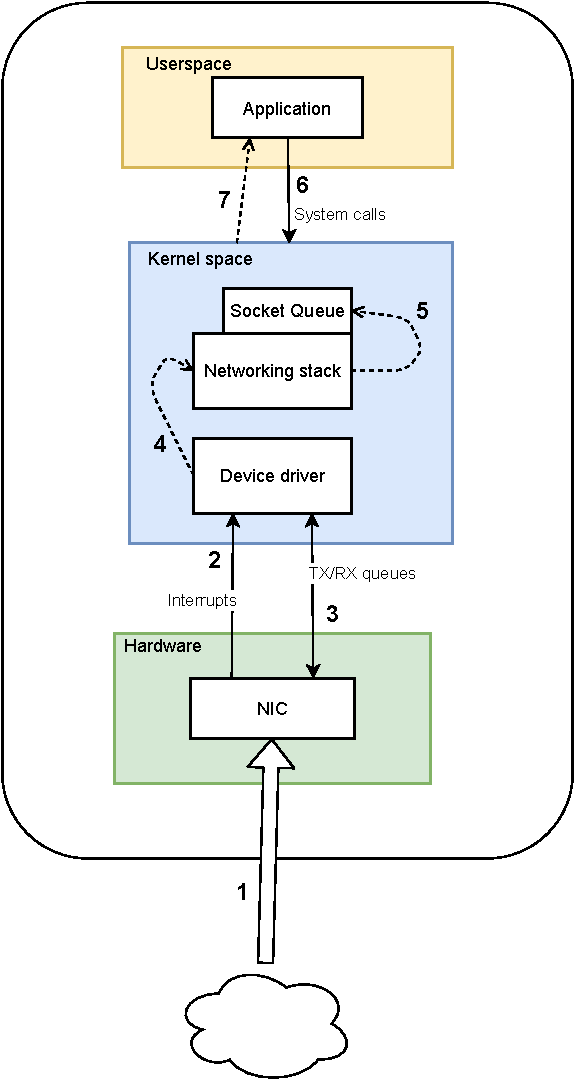
\includegraphics{figures/PDF/receive_path}
    \caption[System overview of hardware to application for receiving a packet.]{System overview of hardware to application for receiving a packet. Path is as follows: 1. remotely a packet is sent and recieved by NIC. 2. Hardware interrupt to the device drive, indicating new packet. 3. Device driver dequeues packet in RX queue. 4. Networking stack processes packet. 5. Packet is enqueued in queue assosiated with the socket. 6. Application performs a read system call, and performs \textit{epoll\_wait} if necessary. 7. Packet is copied and consumed by application.}
    \label{fig:linux_packet}
\end{figure}


Figure \ref{fig:linux_packet} shows the path a receiving packet takes inside a Linux system.
Packet is processed by CPU, and system calls and memory copies needed between stacks and queues.

\section[RDMA]{RDMA}\label{sec:rdma}
Remote Direct Memory Access (RDMA) address the issues of linux sockets, providing lower latency, less CPU overhead, and potentially higher throughput.
RDMA has been used in super computers for many years, however recently have seen significant improvements.
RDMA capable network cards (RNICs) have seen lowering in cost \cite{kalia2016design}, which made this an appealing improvement to data center networking.

RDMA achieves this low latency by offloading the network processing onto the RNIC, bypassing CPU and kernel entirely.
As shown in section \ref{sec:linux-sockets} and figure \ref{fig:linux_packet} above, the Linux kernel has an extensive route, from application to NIC to network, including system calls and memory copies.
With RDMA, a zero-copy memory access can be realised through DMA and programmable IO (PIO) operations, which can be seen in \ref{fig:send_recv_drawing}.
Furthermore, RDMA offloads packet processing to the RNIC, freeing CPU cycles for other tasks.
This makes RDMA a compelling technology for latency sensitive workloads, like KV-store, making remote memory operations possible and perform near to local memory operation speeds.

\subsection{Queue Pairs}\label{subsec:queue-pairs}
RDMA is largely based around the notion of a queue pair (QP).
These consist of a send and receive queue, these are the essence of performing network operations.
These queues can be seen as the receive and transmit queue (RX and TX respectively) in classical NIC, however are bound per QP instead of being shared system wide.
A QP is similar to a linux socket, as these are used to send and receive data.
A work request (WR) is a type of command that tells the RNIC what task to perform and which memory locations are needed, these are passed to the RNIC via PIO operations.
Every WR placed either in the send or receive queue will be consumed in the same order as placed in the queue, similarly for completions of WR's.
This is important when dealing with unreliable transportation, as will be explained in \ref{subsec:transportation-types}.

Queue pairs are also linked with a completion queue (CQ).
This queue is used as a notification queue, with the status of WR's.
For signalled WR's, a completion event will be passed from RNIC to CPU, thus minor CPU involvement.


For RDMA operations like \textit{READ} and \textit{WRITE} this would include the remote address to be accessed, with two-sided verbs such as \textit{SEND} and \textit{RECV} this is accompanied by a buffer for which DMA operations can take place.

\subsection{Transportation types}\label{subsec:transportation-types}
RDMA can make use of several transport protocols, each having their trade-offs.
Simply put, there are three main and supported transport types: reliable connection (RC), unreliable connection (UC), and unreliable datagram (UD).

Firstly, unreliable protocols do not make use of ACK/NAK packets, while this is used for reliable, this could result in packet loss and unordered packets.
However, it has been shown that this rarely occurs\cite{kalia2014using, kalia2016fasst}.
Additionally, this could require application retransmission handling.
With reliable protocol this is process is done by the RNIC, without OS or application involvement.

As stated in the name, RC and UC need a connection between queue pairs (QP).
Only one QP can be connected to another QP.
Contrasting this, unreliable datagram (UD) do not require a connection.
This meaning that a UD QP can communicate with any other UD QP.
UD therefore can make efficient use of a one-to-many network topology or application.
Every QP has to be held by RNIC in cache, which is limited in space\cite{qiu2018toward}.
At large number of QP's, this might not be able to be cached, thus causing cache misses when switching between all QP's.
This cache miss would diminish performance, as QP metadata must be retrieved from main memory.
Data center workloads typically run with many connected machines\cite{vasudevan2009safe}.
If a connection oriented transport type is used in such use cases, performance could be limited\cite{kalia2016fasst}.

UD requires an address handler (AH) to be passed along with its WR's.
AH hold the relevant data for routing a packet to its destination.
The destination does not need to be a QP, but could also be a multicast group.
Multiple clients can listen on the same channel, this is can be applied in applications where the same data can be used by multiple clients.
An AH can be created from a previous work completion (WC), or via metadata exchange, see \ref{subsec:connecting-qp's}.

UD is limited however to a maximum transmission unit (MTU) of 4KB, as can be seen in table \ref{tab:transport-verb}.
Beyond this 4KB, the message is divided into several packets.
This strongly contrasts the 2 GB available for RC and UC.
This has to be taken into account on a per-application bases.
In the case of this thesis, 4 KB is sufficient message size for KV-stores.
Frey and Alonso have comprised a list of application and if it is suitable for RDMA\cite{frey2009minimizing}.

\subsection{Verbs}\label{subsec:verbs}
To interact with RNICs, RDMA uses so-called "verbs" to execute specific types of instructions.
Some of which are: read, write, send, and receive.
Read and write (\textit{READ} and \textit{WRITE}) follow so-called memory semantics, while send and receive (\textit{SEND} and \textit{RECV}) follow channel semantics.
Memory semantics require the destination memory address to be known.
This meaning, to be able to perform a RDMA read of a remote memory location, the memory address of the requested memory needs to be known.

Channel semantics are similar to socket, in the sense that the remote memory address does not need to be known.
However, to perform a \textit{SEND} operation, the receiving end must post a \textit{RECV} WR before the \textit{SEND} WR is sent, this is called pre-posting.
This tells the server's RNIC which memory location the application expects the next incoming message to be place.

Not all verbs are available to every QP type.
Table \ref{tab:transport-verb} summarizes the transportation type and which verb is available.

\begin{table}
    \centering
    \begin{tabular}{l| p{2cm} lll|r}
        \toprule
         & \textbf{Application verb} & & & & \\
         & \textbf{SEND} & \textbf{RECV} & \textbf{READ} & \textbf{WRITE} & \textbf{MTU} \\
        \midrule
        \textit{RC} & YES & YES & YES & YES & 2 GB \\
        \textit{UC} & YES & YES & NO & YES & 2 GB \\
        \textit{UD} & YES & YES & NO & NO & 4 KB \\
        \bottomrule
    \end{tabular}
    \caption{Verbs available to each transportation type}
    \label{tab:transport-verb}
\end{table}

\subsection{Connecting Queue Pairs}\label{subsec:connecting-qp's}
Establishing a connection between QP's involves exchanging metadata related to the QP.
This can be done via a known QP, or via traditional networks, using for example TCP.
However, in some cases, a classical ethernet NIC is not available.
In these circumstances, a known QP can be used.
This is available by the Communication Manager (CM)\cite{mellanox_prog_guide, rdmamojo}.

Unconnected datagrams also require metadata exchange.
Data such as QP number, and physical port, which is are needed to create AH, or join a multicast group.
This can be achieved in the same way as with connected protocols.

\subsection{Programming with RDMA}\label{subsec:programming-with-rdma}

\begin{figure}
    \centering
    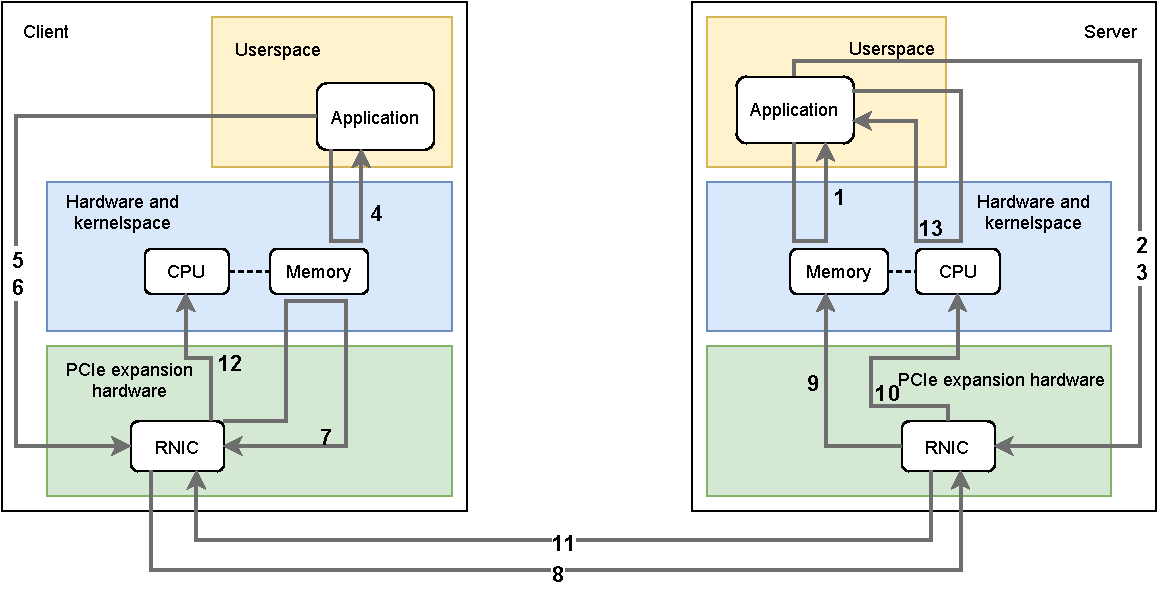
\includegraphics[width=\columnwidth]{figures/PDF/RDMA_SEND_RECV_drawing}
    \caption[Process overview of \textit{SEND} and \textit{RECV}.]{Process overview of pre-posting receive and send from client to server. Numbered arrows have a corresponding function described in \ref{subsec:programming-with-rdma}. Looping arrows such as 1 or 7, indicate memory fetching/polling.}
    \label{fig:send_recv_drawing}
\end{figure}

Unlike traditional sockets, much of RDMA's programming API allows for more control, thus more detailed optimizations can be implemented.
This interface is developed and supported by the OpenFabrics Alliance\cite{openfab}.
The cost of this is the need for more memory management in userspace, which otherwise would be done by the kernel.
In this subsection, this open interface will be discussed, what functions are needed to be done to make use of RDMA, and what happens internally.
For this, figure \ref{fig:send_recv_drawing} illustrates the process of an RC QP connection, and \textit{SEND} and \textit{RECV} operation, from client to server.
It is assumed that client and server have successfully made a protection domain (PD), QP, and connect or exchanged data for these QP's, see section \ref{subsec:connecting-qp's} on how this can be done.
Protection domains are used to separate resources, such as memory regions, QP's, and AH.

The numbered arrows in figure \ref{fig:send_recv_drawing} correspond to the following:

\begin{enumerate}
    \item The server application should allocate memory for its receiving buffer.
    \item This buffer should be registered in the RNIC under the PD used for this application.
    By registering memory, a page table entry will be held in RNIC's cache, as shown with the corresponding dashed line.
    \item Server pre-posts a receive.
    This is needed to be able to receive before the client will send.
    Usually this is done just before connecting, this way even if the receiving end lags behind, the RNIC will be ready to receive.
    \item Client allocates the buffer that will be sent.
    \item Also registering this buffer.
    This can be done while the server is completing steps 1 and 2.
    \item Posting a \textit{SEND} WR to the RNIC.
    This signals the RNIC that a given registered memory address will be sent via its QP.
    \item The RNIC fetches this data in memory using DMA.
    \item In step 8, this data is then sent over the network to the server.
    \item The server's RNIC receives this data and performs an DMA operation to the buffer given by its \textit{RECV} WR.
    \item RNIC notifies with a completion event to the CPU, that it has a new event in its CQ.
    \item RNIC also sends a completion event to the client, in the case of reliable connection.
    \item This completion event is passed along to the CPU, to signal a waiting thread.
    \item The server can poll on the CQ, this tells the application that the \textit{RECV} request has been completed, and can now be read with the same data as was in the clients buffer.
\end{enumerate}

For more insight in which functions are avaliable, see RDMA programming guide\cite{mellanox_prog_guide} or the OpenFabric Alliance\cite{openfab} which develop kernel bypassing API for RDMA aware networks.
% ---------------------------------------------------------------------------
% ----------------------- end of thesis sub-document ------------------------
% ---------------------------------------------------------------------------

% this file is called up by thesis.tex
% content in this file will be fed into the main document

\chapter{Design} % top level followed by section, subsection


% ----------------------- paths to graphics ------------------------

% change according to folder and file names
\ifpdf
    \graphicspath{{7/figures/PNG/}{7/figures/PDF/}{7/figures/}}
\else
    \graphicspath{{7/figures/EPS/}{7/figures/}}
\fi


% ----------------------- contents from here ------------------------
% 

\dots



% ---------------------------------------------------------------------------
% ----------------------- end of thesis sub-document ------------------------
% ---------------------------------------------------------------------------

% this file is called up by thesis.tex
% content in this file will be fed into the main document

\chapter{Evaluation}\label{ch:evaluation} % top level followed by section, subsection


% ----------------------- paths to graphics ------------------------

% change according to folder and file names
\ifpdf
    \graphicspath{{figures/PNG}}
\else
    \graphicspath{{7/figures/EPS/}{7/figures/}}
\fi


% ----------------------- contents from here ------------------------
% 
In this section, the experimental results are presented.
%First a baseline of RDMA performance on DAS is given.
%This will be used to compare a KV store use case to maximum performance that can be achieved on DAS.
The RDMA transportation types are compared within and against the baseline TCP implementation.
Throughput and latency are mainly used to analysis the scalability of these transportation types.
The same raw data is used for both measurements, thus can be put alongside each other.

In short, the results show:
\begin{itemize}
    \item Throughput reaches an equilibrium with all transportation types up to 30 clients.
    UD performs best, with a maximum throughput of roughly 400 kilo-tasks/sec.
    Further details are given in section \ref{sec:throughput-analysis}.
    \item Latency increases across all transportation types, with increased number of clients.
    Results are inversely comparable to throughput, again with UD performing best, with a latency of roughly 0.058 ms at 30 clients TODO ACCURATE.
    Section \ref{sec:latency:analysis} delves deeper.
\end{itemize}

To recall the benchmarking setup:
Ten million tasks are divided equally between \textit{n}-clients.
A task is defined as a request and response, and are equal to two operations.

\section{Throughput analysis}\label{sec:throughput-analysis}
We compare the average throughput between TCP, RC, and UD with up to 30 clients.
From figure \ref{fig:throughput-30}, the maximum average throughput is observed to be roughly 205 kilo-tasks/sec for TCP, 251 kilo-tasks/sec for RC, both at 30 clients, and 399 kilo-tasks/sec for UD at 25 clients.
RC shows a mere 22.8\% maximum improvement over TCP.
UD in turn offers a significant gain of 94.8\% over TCP.
\begin{figure}
    \centering
    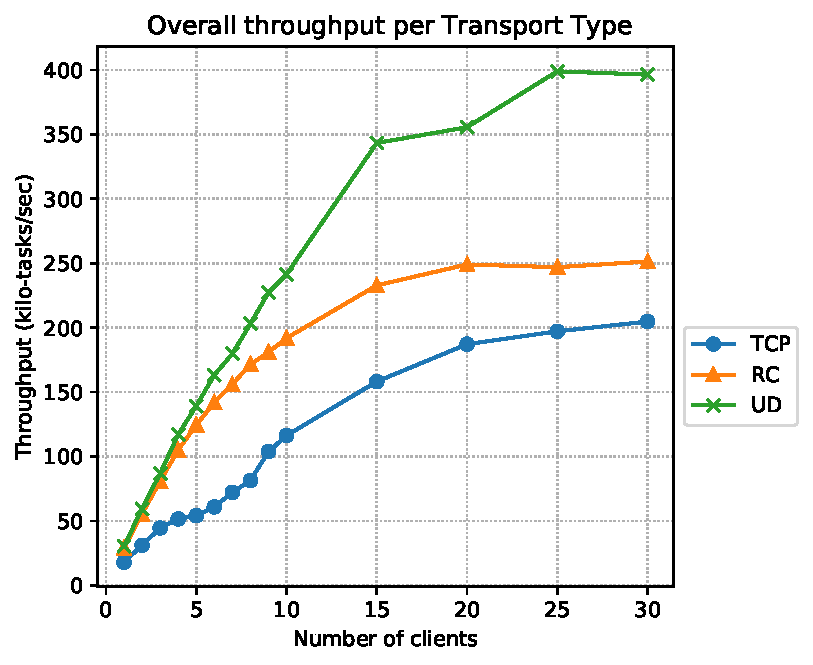
\includegraphics[width=\columnwidth]{figures/PDF/Throughput_30}
    \caption{Throughput of clients executing 10 million operations}
    \label{fig:throughput-30}
\end{figure}

\subsection{Scalability rate}\label{subsec:scalability-rate}
It can be observed from figure \ref{fig:throughput-30} that all transportation types scale up to roughly 20 clients before settling.
UD outperforms the other types, in both throughput and initial rate of scalability.
A near linear scalability rate can be seen in the first 15 clients for UD.
This is due the addition of threads for every new client.
Since all these threads are actively working for all clients, this linear increase is to be expected.
For the first 10 clients, UD increases its throughput by 23.4 kilo-tasks/sec per additional client.
Compare this with 18.1 for RC and 10.9 kilo-tasks/sec for the baseline TCP.
This shows strong scalability for UD with small number of clients.
It is unclear from this graph if UD continues to scale beyond 30 clients.

\subsection{Similarities between RC and TCP}
It can also be seen in figure \ref{fig:throughput-30} that RC is similar to TCP in scalability.
With both being a connection oriented protocol, each server thread being tied to a client, it shows similar performance.
The benefits of RDMA do reflect in these results, with the throughput of RC being on average 59.7 kilo-tasks/sec above TCP.
Both protocol stabilizing after roughly 20 clients, with less than 5\% change for TCP and less than 2\% for RC.

\subsection{Fairness between clients}
TODO GENERATE GRAPH FOR THIS

\section{Latency analysis}\label{sec:latency:analysis}
An important factor to KV store is their quick response time, and therefore this should ideally scale similarly, preferably better, than throughput.
RDMA offers fast response time due to the lack of CPU and kernel involvement.
To see how this is translated per transportation type, the average latency of all 10 million tasks were measured, from request sent to response received.
Results can be seen in figure \ref{fig:latency-30}.
Along with the average latency, the first and third quartile are shown, to analyze the variation of latencies.

\begin{figure}
    \centering
    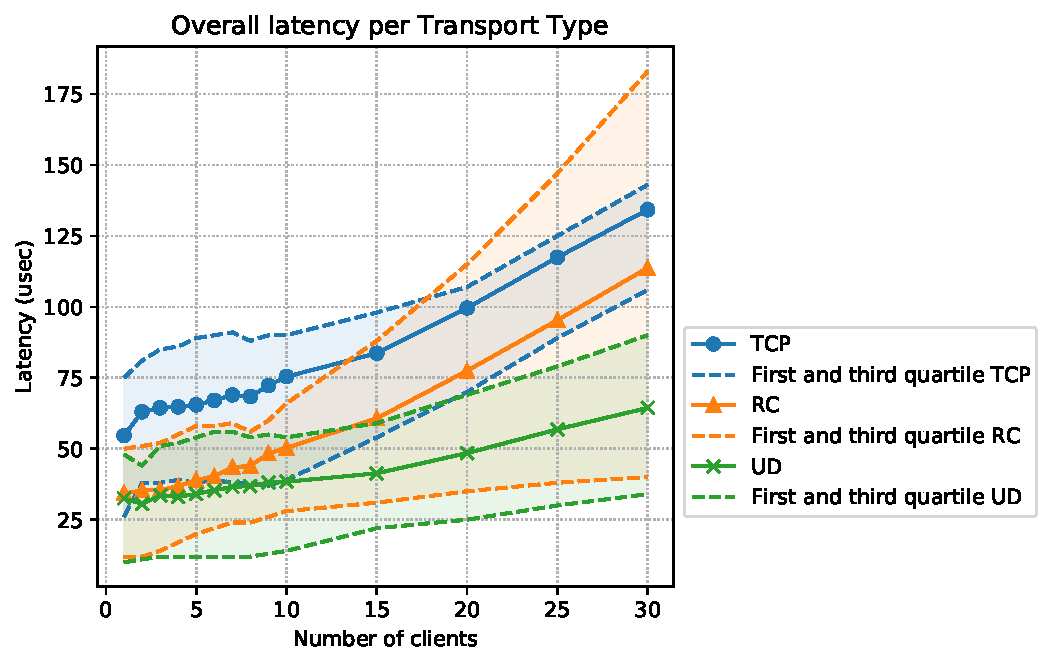
\includegraphics[width=\columnwidth]{figures/PDF/Latency_avg_30}
    \caption{Latency of clients executing 10 million operations}
    \label{fig:latency-30}
\end{figure}

The latency between protocols is an inverse reflection of the throughput graph, scaling and overall performance.
Similarly, TCP performed worst, with an average latency of 0.135ms TODO ACCURATE NUMBER at 30 clients.
RC following the same path as TCP and hits an average of 0.11ms, also at 30 clients.
UD again performing best, reaching 0.06ms on average.
This is an order of magnitude more than has been found in FaSST\cite{kalia2016fasst}, HERD\cite{kalia2014using}, and what should be theoretically possible.
This could be due to lock contention with shared QP, and poor performance of KV store.
A further examination of this could support this.

Similarly to throughput, UD scales relatively well, while RC and TCP scale linearly.
A near uniform latency for the first 15 clients, afterwards a gradual slope, compared to TCP and RC.

\subsection{Variation from average}
In figure \ref{fig:latency-30} the variation is given in form of first and third quartile.
It can be seen that TCP and UD have a constant, a small, variation.
TCP is skewed towards higher latencies at 30 clients, while UD, and RC, stay normally distributed throughout.
RC has a rapidly increasing variation.
This is concerning for scalability and consistency, and could possibly be due to context switching.

\subsection{All 30 clients and per operation latency}\label{subsec:all-30-clients-and-per-operation-latency}
Figure TODO ADD REFERENCE TO GRAPH OF ALL 3 PER CLIENT LATENCY delves deeper into the details of the variation in latency.
Within all protocols there are outliers and spikes in latency.
Surprisingly, TCP has the least varying results, despite the few initial spikes.

\subsection{RDMA multiple QP's causing cache misses and context switching}
In section \ref{subsec:transportation-types} the issue with holding multiple QP's within the RNIC, has been discussed.
The RNIC needs to perform context switching when changing QP.
As the number of QP's increase, like with connection oriented transport types, the number of context switches needed increases.
Along this, the chance of cache misses are also increased.
This decreases the performance, with increased latency, and in throughput as shown here.
With context switching, a large delay occurs, and harms the performance per client, but also of the overall network.
For this reason, for large number of clients, a one-to-one QP is not advisable.

\subsubsection{Cache misses as increased variation for RC}
Furthermore, cache misses occur more often at the starting phase of KV store operations, as can be seen in section TODO PER CLIENT LATENCY above.
RC has consistently higher latency (0.75ms) for some clients at the start.
Initially it was thought to be retransmissions, however for this was set to 67.1ms.
Since this only occurs to some clients, and not all, this could be a result from the aforementioned context switching and RNIC cache misses.
At the start of operations, worker threads are operating in sync.
This would result in RNIC processing multiple WR's concurrently.
Some QP's will be cached and experience little cache misses throughout the starting phase, while others would encounter cache misses repeatedly.
Once threads are out of sync and KV store operation latency increases (due to the increasing size of the hash table), the cache misses will occur for all QP's.
This can be seen in figure TODO, as the latency in the final phase is randomized and less constant, compared to the starting phase.

With cache misses, latency per client varies, as some QP's would require further lookup after cache miss.
This effect can be seen in figure \ref{fig:latency-30}, as increasing number of clients, and therefore QP's, increases the variation dramatically.
Further investigation into cache misses would support these claims, this has not been done for this thesis.

% ---------------------------------------------------------------------------
% ----------------------- end of thesis sub-document ------------------------
% ---------------------------------------------------------------------------

% this file is called up by thesis.tex
% content in this file will be fed into the main document

\chapter{Related Work}\label{ch:related-work} % top level followed by section, subsection


% ----------------------- paths to graphics ------------------------

% change according to folder and file names
\ifpdf
    \graphicspath{{7/figures/PNG/}{7/figures/PDF/}{7/figures/}}
\else
    \graphicspath{{7/figures/EPS/}{7/figures/}}
\fi


% ----------------------- contents from here ------------------------
%
\section{HERD}
There are several proposed RDMA KV store designs.
One of which, HERD \cite{kalia2014using}, uses a combination of transport types.
HERD uses RDMA \textit{WRITE} over UC for requests and \textit{SEND} over UD for responses.
Kalia et. al. have shown that incoming \textit{WRITE}s offers lower latency and higher throughput compared to \textit{READ}.
Outgoing \textit{WRITE}s have also been shown to not scale well, making this unadvisable for sending responses.

HERD out performs the RDMA KV store presented in this thesis significantly.
This could due to multiple factors:
\begin{itemize}
    \item HERD has implemented some optimizations towards prefetching before posting a \textit{SEND} WR.
    With this they have observed roughly 30\% improvement, in the best case comparison (2 random memory accesses at 4 CPU cores.)
    \item Making use of one-sided \textit{WRITE} for requests, bypassing the CPU.
    \item Using inlined data for key.
    Inlining small payloads decreases latency as there is no need for a DMA operation.
\end{itemize}

However, Kalia et. al. stated that performance should be comparable to \textit{SEND}/\textit{SEND}, given that inlining is possible.
It was found that for a large number of clients and/or requests, the round-robin polling used, is inefficient.
With 1000s of clients, a \textit{SEND}/\textit{SEND} design would scale better than the \textit{WRITE}/\textit{SEND} used in HERD.



% ---------------------------------------------------------------------------
% ----------------------- end of thesis sub-document ------------------------
% ---------------------------------------------------------------------------

% this file is called up by thesis.tex
% content in this file will be fed into the main document

\chapter{Future improvements}\label{ch:future-improvements} % top level followed by section, subsection


% ----------------------- paths to graphics ------------------------

% change according to folder and file names
\ifpdf
    \graphicspath{{7/figures/PNG/}{7/figures/PDF/}{7/figures/}}
\else
    \graphicspath{{7/figures/EPS/}{7/figures/}}
\fi


% ----------------------- contents from here ------------------------
%
\section{Experimental transport types}
Current transportation types all have advantages and disadvantages.
Reliable transport has advantages being predictable packet behavior.
However, as has been shown in this thesis, connection transports (such as RC) have scalability issues, due to the RNIC caching issues with increasing number of QP's.
Dynamically Connected Transport (DCT) is, currently, an experimental transport type which addresses these issues.
DCT has a connection based design, while only requiring one QP.
This is achieved by dynamically connecting and disconnecting with remote QP's, which would introduce additional latency with short-lived clients, or when dealing with concurrent large number of clients.

\section{Optimizations}
Currently, no optimizations are used to improve performance.
Since this thesis focused on performance across transport types, this needed to remain consistent throughout.
Optimizations, such as those used in HERD, improve performance significantly.
Other optimizations can be found in Kalia et. al. paper on design guidelines and possible optimizations\cite{kalia2016design}.

This thesis has shown the potential of using UD as scalable and high throughput transport type for RDMA KV stores, however this could be improved further.
One improvement is to have multiple groups of clients, each with a single QP.
This has been shown to be effective in ScaleRPC\cite{chen2019scalable}.
Grouping clients reduces RNIC cache contention, by limiting the number of worker threads competing for cache. TODO
However, like with RC and UC, using multiple QP's increases context switching, which harms performance.
ScaleRPC have proposed solutions by "warming up" QP's.


% ---------------------------------------------------------------------------
% ----------------------- end of thesis sub-document ------------------------
% ---------------------------------------------------------------------------

% this file is called up by thesis.tex
% content in this file will be fed into the main document

\chapter{Conclusion}\label{ch:conclusion} % top level followed by section, subsection


% ----------------------- paths to graphics ------------------------

% change according to folder and file names
\ifpdf
    \graphicspath{{7/figures/PNG/}{7/figures/PDF/}{7/figures/}}
\else
    \graphicspath{{7/figures/EPS/}{7/figures/}}
\fi


% ----------------------- contents from here ------------------------
%
RDMA has been shown to be a promising advancement for key values stores.
The low latency that RDMA brings with it, opens op new possibilities and improved performance.
RDMA also requires more design decision to be made, which transportation protocol to use, which optimizations to use, and which verbs to use.
In this thesis, the transportation protocols RC and UD have been compared, on performance, to TCP.

\textbf{RQ1:} In industry, KV stores require to be scalable and low latency.
Connection based transportation (RC and UC) put stress on RNIC when using large number of clients, hindering performance with respect to throughput and scalability.
RC has similar scalability to TCP, with a near 60 kilo-tasks/sec increase in throughput across all number of clients.
Best performing transportation type is UD, with close to 400 kilo-tasks/sec throughput and 64 $\mu$sec at 30 clients.
It has been shown that UD offers a 58.7\% improvement in throughput against RC, and 45.5\% improvement in latency.
For scalability UD is recommended to use, as this offers the best overall performance and sustains this up to 30 clients, and has the potential for optimizations to further improve performance.

\textbf{RQ2:} The advantages and disadvantages present with the different transportation types impact the KV store design choices.
In context of KV stores, UD is a compelling transportation type, however does not offer RDMA verbs such as \textit{READ} and \textit{WRITE}, which could offer for improved performance.
UD also allow for more optimizations, due to their one-to-many QP.
UD performance in this thesis have found to be limited.
Multiple UD QP's along with client grouping could continue scalability further.
Connection based transportation types are limited by one-to-one QP, although also have some room for improvements.


% ---------------------------------------------------------------------------
% ----------------------- end of thesis sub-document ------------------------
% ---------------------------------------------------------------------------
%\include{3_materials&methods/materials_methods}						
%\include{4_analysis&results/analysis&results}	

%\include{5_discussions/discussions}

%% this file is called up by thesis.tex
% content in this file will be fed into the main document

\chapter{Conclusion}\label{ch:conclusion} % top level followed by section, subsection


% ----------------------- paths to graphics ------------------------

% change according to folder and file names
\ifpdf
    \graphicspath{{7/figures/PNG/}{7/figures/PDF/}{7/figures/}}
\else
    \graphicspath{{7/figures/EPS/}{7/figures/}}
\fi


% ----------------------- contents from here ------------------------
%
RDMA has been shown to be a promising advancement for key values stores.
The low latency that RDMA brings with it, opens op new possibilities and improved performance.
RDMA also requires more design decision to be made, which transportation protocol to use, which optimizations to use, and which verbs to use.
In this thesis, the transportation protocols RC and UD have been compared, on performance, to TCP.

\textbf{RQ1:} In industry, KV stores require to be scalable and low latency.
Connection based transportation (RC and UC) put stress on RNIC when using large number of clients, hindering performance with respect to throughput and scalability.
RC has similar scalability to TCP, with a near 60 kilo-tasks/sec increase in throughput across all number of clients.
Best performing transportation type is UD, with close to 400 kilo-tasks/sec throughput and 64 $\mu$sec at 30 clients.
It has been shown that UD offers a 58.7\% improvement in throughput against RC, and 45.5\% improvement in latency.
For scalability UD is recommended to use, as this offers the best overall performance and sustains this up to 30 clients, and has the potential for optimizations to further improve performance.

\textbf{RQ2:} The advantages and disadvantages present with the different transportation types impact the KV store design choices.
In context of KV stores, UD is a compelling transportation type, however does not offer RDMA verbs such as \textit{READ} and \textit{WRITE}, which could offer for improved performance.
UD also allow for more optimizations, due to their one-to-many QP.
UD performance in this thesis have found to be limited.
Multiple UD QP's along with client grouping could continue scalability further.
Connection based transportation types are limited by one-to-one QP, although also have some room for improvements.


% ---------------------------------------------------------------------------
% ----------------------- end of thesis sub-document ------------------------
% ---------------------------------------------------------------------------
          
%% this file is called up by thesis.tex
% content in this file will be fed into the main document

%: ----------------------- name of chapter  -------------------------
\chapter*{Appendix} % top level followed by section, subsection


%: ----------------------- paths to graphics ------------------------

% change according to folder and file names
\ifpdf
    \graphicspath{{X/figures/PNG/}{X/figures/PDF/}{X/figures/}}
\else
    \graphicspath{{X/figures/EPS/}{X/figures/}}
\fi

%: ----------------------- contents from here ------------------------
\includepdf[pages=1-5]{CodesTable} 
\includepdf[pages=1-4]{InterviewQuestions}





% ---------------------------------------------------------------------------
%: ----------------------- end of thesis sub-document ------------------------
% ---------------------------------------------------------------------------


      
            
% --------------------------------------------------------------
%:                  BACK MATTER: appendices, refs,..
% --------------------------------------------------------------

% the back matter: appendix and references close the thesis


%: ----------------------- bibliography ------------------------

% The section below defines how references are listed and formatted
% The default below is 2 columns, small font, complete author names.
% Entries are also linked back to the page number in the text and to external URL if provided in the BibTex file.

% PhDbiblio-url2 = names small caps, title bold & hyperlinked, link to page 
%\begin{multicols}{2} % \begin{multicols}{ # columns}[ header text][ space]
%\begin{tiny} % tiny(5) < scriptsize(7) < footnotesize(8) < small (9)

%\bibliographystyle{Latex/Classes/PhDbiblio-url2} % Title is link if provided
\bibliographystyle{plainnat}
\renewcommand{\bibname}{References} % changes the header; default: Bibliography

\bibliography{8_references/thesis} % adjust this to fit your BibTex file

%\end{tiny}
%\end{multicols}



% --------------------------------------------------------------
% Various bibliography styles exit. Replace above style as desired.

% in-text refs: (1) (1; 2)
% ref list: alphabetical; author(s) in small caps; initials last name; page(s)
%\bibliographystyle{Latex/Classes/PhDbiblio-case} % title forced lower case
%\bibliographystyle{Latex/Classes/PhDbiblio-bold} % title as in bibtex but bold
%\bibliographystyle{Latex/Classes/PhDbiblio-url} % bold + www link if provided

%\bibliographystyle{Latex/Classes/jmb} % calls style file jmb.bst
% in-text refs: author (year) without brackets
% ref list: alphabetical; author(s) in normal font; last name, initials; page(s)

%\bibliographystyle{plainnat} % calls style file plainnat.bst
% in-text refs: author (year) without brackets
% (this works with package natbib)


% --------------------------------------------------------------

% according to Dresden med fac summary has to be at the end
%
% Thesis Abstract -----------------------------------------------------


%\begin{abstractslong}    %uncommenting this line, gives a different abstract heading
\begin{abstracts}        %this creates the heading for the abstract page

    Seemingly ever growing tech giants, such as Facebook, Amazon and Google, require fast, reliable and scalable key-value storage (KV-store) to serve product recommendations, user preferences, and advertisements.
    Past advancements of KV-stores have focussed on improving these underlying data structures.
    Remote direct memory access (RDMA) networks have increasingly become more popular in commercial and academic data centers.
    This relatively new technology offer lower latency and higher throughput performance compared to tradition sockets and network interface cards (NIC).
    Scalability performance of RDMA transportation protocols is less known, previous work focused on RDMA verb choice.

    This paper focuses on this gap, evaluating scalability performance of RDMA transportation types.
    These findings will be used to give recommendation for RDMA KV-store implementations.
    Macro-level benchmarks have been conducted, with realistic KV-store workloads.
    It has been found that RDMA offers a significant improvements compared to TCP.
    UD has shown to perform best, with 94.8\% throughput improvement over TCP, and 58.7\% improvement over RC.
    All the while offering consistent and gradually increasing latency up to 30 clients, reaching a maximum average latency of 64 $\mu$sec.
    Additionally, scalability issues of RC have been shown, and is not recommended in a KV-store application.

\end{abstracts}
%\end{abstractlongs}


% ---------------------------------------------------------------------- 


%: Declaration of originality
%\include{8_backmatter/declaration}



\end{document}
